\documentclass[12pt]{ut-thesis}

% ----------------------------------------------------------------------------------------------------------------------------------------
% USEPACKAGE DECLARATIONS
% ----------------------------------------------------------------------------------------------------------------------------------------

%\includeonly{./sections/reionization}

\usepackage{amsmath}
\usepackage{amssymb}
\usepackage{aas_macros}
\usepackage{natbib}
\usepackage{html}
\usepackage{graphicx}
\usepackage{rotating}
\usepackage{tabularx}
\usepackage{pdflscape}
\usepackage{afterpage}
\usepackage{capt-of}
\usepackage{setspace}
\doublespacing 


%\usepackage[figuresleft]{rotating}

% ----------------------------------------------------------------------------------------------------------------------------------------
% AUTHOR INFORMATION
% ----------------------------------------------------------------------------------------------------------------------------------------

\degree{Doctor of Philosophy}
\department{Astronomy and Astrophysics}
\gradyear{2016}
\author{Liam Dean Connor}
\title{Long Wavelength Astrophysics}

% ----------------------------------------------------------------------------------------------------------------------------------------
% COMMANDS AND DEFINITIONS
% ----------------------------------------------------------------------------------------------------------------------------------------

% Put here all other formatting commands that belong in the preamble. In particular, you should put all of 
% your \newcommand's, \newenvironment's, \newtheorem's, etc. (in other words, all the global definitions 
% that you will need throughout your thesis) in a separate file and use "\input{filename}" to input it here.
\input{commands}

% Table of contentds depth (0 = chapter, 1 = section, 2 = subsection, 3 = subsubsection, etc.)
\setcounter{tocdepth}{2}

% Make each page fill up the entire page.
\flushbottom

% ==============================================================================
% PRELIMINARY CONTENT
% ==============================================================================

\begin{document}

% This sets the page style and numbering for preliminary sections.
\begin{preliminary}

% This generates the title page from the information given above.
\maketitle

% There should be NOTHING between the title page and abstract.  However, if your document 
% is two-sided and you want the abstract _not_ to appear on the back of the title page, then uncomment 
% the following line.
% \cleardoublepage

% ----------------------------------------------------------------------------------------------------------------------------------------
% ABSTRACT
% ----------------------------------------------------------------------------------------------------------------------------------------

\begin{abstract} % At most 350 words for Ph.D.

\end{abstract}

% Anything placed between the abstract and table of contents will appear on a separate page since the 
% abstract ends with \newpage and the table of contents starts with \clearpage.  Use \cleardoublepage
% for anything that you want to appear on a right-hand page.

% ----------------------------------------------------------------------------------------------------------------------------------------
% DEDICATION
% ----------------------------------------------------------------------------------------------------------------------------------------

%\begin{dedication}
\vspace*{\fill}
\begin{center}
{\em }%To Pop and my infinitely supportive parents}
\end{center}
\vfill
%\end{dedication}

\newpage % Force separate pages for dedication and acknowledgements


% ----------------------------------------------------------------------------------------------------------------------------------------
% ACKNOWLEDGEMENTS
% ----------------------------------------------------------------------------------------------------------------------------------------

\begin{acknowledgements}
 % The research presented in this thesis sample the work 
 % I have done over the last five years, which has 
 % ranged from what felt like mathematical musings to software development  
 % to on-site hardware work. This is because both of my supervisors, 
 % Ue-Li Pen and Keith Vanderlinde, possess end-to-end expertise, 
 % with firm understanding of the physics in which we are interested 
 % as well as the steps required to make such measurements come to fruition;
 % needless to say this thesis would not have been possible without them. 
 % A similarly insightful supervisory figure was Richard Shaw, 
 % whose ease with signal processing, statistics, and computing 
 % was greatly appreciated in my first few years of graduate school. 

 % On the CHIME team, I was lucky enough to work closely 
 % with such world-class experimental cosmologists as Mark Halpern 
 % and Gary Hinshaw. Tom Landecker was an irreplaceable source 
 % of knowledge and wisdom during my many 
 % visits to DRAO, acting as the token radio astronomer in a 
 % large radio astronomy project. I would also thank my 
 % thesis committee, including Barth Netterfield and Mike Reid. 

\end{acknowledgements}

% ----------------------------------------------------------------------------------------------------------------------------------------
% TABLE OF CONTENTS
% ----------------------------------------------------------------------------------------------------------------------------------------

\tableofcontents

% ----------------------------------------------------------------------------------------------------------------------------------------
% LIST OF TABLES
% ----------------------------------------------------------------------------------------------------------------------------------------

\listoftables

% ----------------------------------------------------------------------------------------------------------------------------------------
% LIST OF FIGURES
% ----------------------------------------------------------------------------------------------------------------------------------------

%\listoffigures

\end{preliminary}

% ==============================================================================
% CHAPTERS
% ==============================================================================

%%%%%%%%%%%%%%%%%%%%%%%%%%%%%%%%%%%%%%%%%%%%%%%%%%%%%%%%%%%%%%%%%%%%%%%%
%%  Put your Chapters here; the easiest way to do this is to keep     %%
%%  each chapter in a separate file and `\include' all the files.     %%
%%  Each chapter file should start with "\chapter{ChapterName}".      %%
%%  Note that using `\include' instead of `\input' will make each     %%
%%  chapter start on a new page, and allow you to format only parts   %%
%%  of your thesis at a time by using `\includeonly'.                 %%
%%%%%%%%%%%%%%%%%%%%%%%%%%%%%%%%%%%%%%%%%%%%%%%%%%%%%%%%%%%%%%%%%%%%%%%%

%\include{./sections/introduction}
\include{./sections/chime}
% \chapter{Beamforming}
\label{chapter:beamforming}
\chaptermark{Beamforming}

% ================================================================================
% CHAPTER OVERVIEW
% ================================================================================

% ======= Liam Notes  ========

\section{Chapter Overview}

This chapter outlines the basic theory behind 
digital beamforming, and describes the commissioning 
of the first beamformer on CHIME Pathfinder. This 
includes the synthesis of several different software packages, 
the implementation of a scheduler, 
and an automated point-source calibration daemon that 
removes drifting instrumental gains in real-time. We will 
also detail early pulsar work and the beamformer's first light. 
This includes the first ever coherent pulsar observations 
taken with CHIME. 
Finally, the creation of an ongoing VLBI FRB search between 
the DRAO and ARO will be outlined, starting with a real-time 
24/7 search of the Pathfinder's synthetic beam. We discuss early 
results, including the false-positive rate and distribution, as 
well as the implications of a non-detection on the FRB brightness 
distribution, $N(S)$.
% ================================================================================
% INTRODUCTION
% ================================================================================

\section{Introduction}

Beamforming is a signal processing technique that allows for 
spatial filtering, and has greatly benefited a diverse set of fields 
from radar and wireless communications to radio astronomy 
\citep{1988IASSP...5....4V}. Whether being used in phased-array RADAR
\citep{2007BAMS...88.1753Z}, 
ultrasonic imaging \citep{macovski1983medical}, or 
wide-band radio astronomy \citep{2013PASA...30....7T}, beamforming 
allows for heightened sensitivity or output to select spatial
modes. This usually involves a sensor (in our case an antenna)
being used alongside a processor (in our case, a computing cluster) 
\citep{1988IASSP...5....4V}. Modern astronomy will benefit greatly from this
technology. 
Beamforming is particularly essential to CHIME. 
The pulsar back-end will rely on
brute-force beamforming in order to track ten sources at a time, 24-7.  
The FRB experiment will FFT-beamform to generate 1024 fan-beams, 
in order to search them in real time for radio transients. Finally, the cosmology 
experiment has always left itself the option of beamforming, whose 
computing cost scales as $N\log N$, as 
an alternative to the full-$N^2$ correlation.
  
% ================================================================================
% THEORY AND IMPLEMENTATION
% ================================================================================
  
\section{Theory and Implementation}
\label{sec:theory}

By coherently combining the voltages of a multi-element array, 
sensitivity can be allocated to small regions of the sky and 
the array's effective forward gain can be increased. The signal 
from each antenna, $x_n$, is multiplied by a complex weight whose 
phases, $\phi_{n}$, are chosen a priori to maximally destructively interfere radio waves 
in all directions but the desired pointing. After applying 
such weights, the signals 
from all antennas are combined to give the formed-beam 
voltage stream, $X_{\rm BF}$.

\begin{equation}
\label{eq-bf_sum}
X_{\rm BF} = \sum_{{n}=1}^N a_n e^{i\phi_{n}} x_n
\end{equation}

\noindent Here $a_n$ are real numbers that can be used as 
amplitude weightings for the antennas. If we define a more 
general complex weighting, $w_n \equiv a_n e^{i\phi_{n}}$, and 
switch to vector notation, Eq.~\ref{eq-bf_sum} becomes,

\begin{equation}
X_{\rm BF} = \mathbf{w} \, \mathbf{x}^{\rm T} .
\end{equation}

\noindent In general, $X_{\rm BF}$ and $\mathbf{x}^{\rm T}$ will be 
functions of time and frequency. This is also true for $\mathbf{w}$,
unless one needs a static, non-tracking beam -- which is the case for the 
CHIME Pathfinder's transient search, described in
Sect.~\ref{vlbi_frb}. We can write this explicitly as follows,


\begin{align}
     \mathbf{w}_{\rm t \nu} &= \left (a_1(\nu) e^{i \phi_1(\nu)}, \, 
     a_2(\nu) e^{i \phi_2(\nu)}, ... \,, \,a_N(\nu) e^{i \phi_N(\nu)} \right )\\
     \mathbf{x}_{\rm t \nu} &= \left ( x_1(\rm{t}, \nu), \, x_2(\rm{t}, \nu), 
     ..., \, x_N(\rm{t}, \nu) \right ).
\end{align}

The voltage stream, $X_{\rm BF}$, is then effectively squared and integrated 
to give a visibility stream. 
In the case of CHIME, $X_{\rm BF}$ corresponds to a single polarization 
so to get the full Stokes information one must compute the 
north-south polarization's autocorrelation, the east-west autocorrelation, 
and their cross-correlation. The Stokes vector can be written as,

% Make sure Stokes stuff is already defined.
\begin{equation}
\mathbf{S} = 
\begin{pmatrix}
I \\ 
Q \\ 
U\\ 
V
\end{pmatrix}
= \begin{pmatrix}
\, X_{\rm ew} X_{\rm ew}^* + X_{\rm ns} X_{\rm ns}^*\, \\ 
\, X_{\rm ew} X_{\rm ew}^* - X_{\rm ns} X_{\rm ns}^* \,\\ 
\, \Re e(X_{\rm ew} X_{\rm ns}^*)\,\\ 
\, \Im m(X_{\rm ew} X_{\rm ns}^*)\,
\end{pmatrix}.
\end{equation}


\subsection{Geometric phase}

We now need to calculate $\phi_n$ across the array.
Ignoring instrumental phases for now, one can compute the geometric 
phases for an antenna by projecting its position vector, $\mathbf{d}_n$, 
onto the pointing vector, $\hat{\mathbf{k}}$. This gives,

\begin{equation}
\label{eqn-phi_n}
\phi_n = \frac{2\pi}{\lambda} \, \mathbf{d}_n \cdot  {\mathbf{\hat{k}}},
\end{equation}

\noindent where we have taken $\mathbf{d}_n$ to be the baseline vector between 
feed $n$ and an arbitrary reference point, and $\phi_n$ is the corresponding 
phase difference. A sketch for this is shown in 
Fig.~\ref{fig-bf_diagram} on page 
\pageref{fig-bf_diagram}.


%trim={<left> <lower> <right> <upper>}
\begin{figure}[!h]
\label{fig-bf_diagram}
\begin{center}
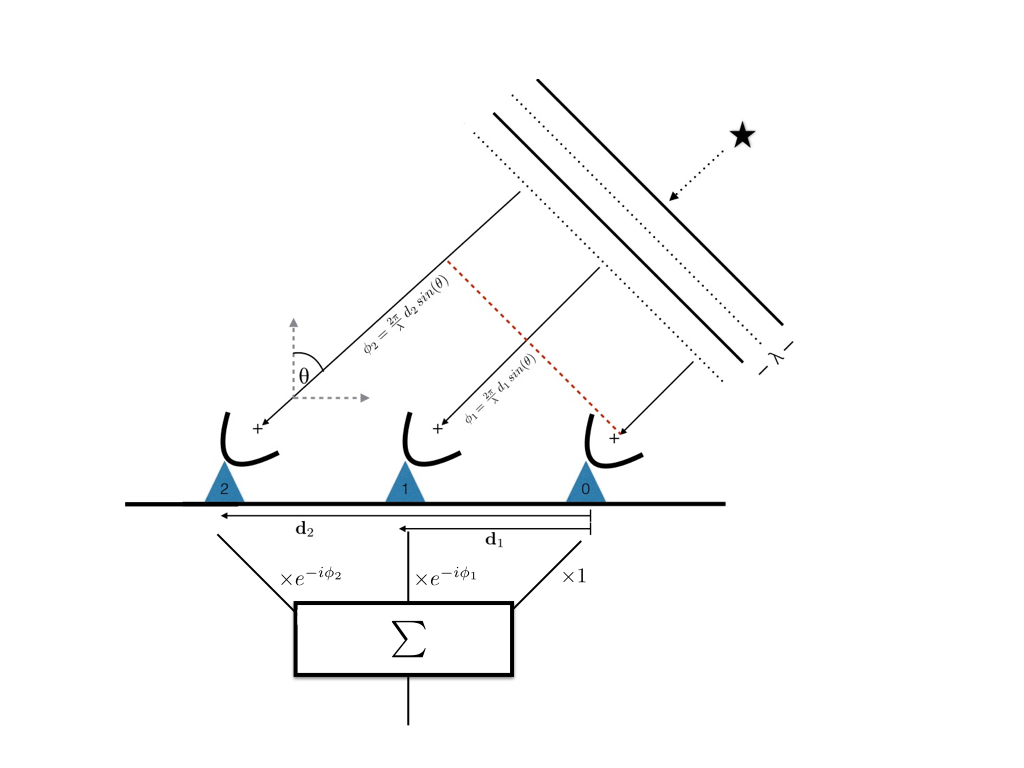
\includegraphics[trim={1.in, 1.in, 2.5in, 1.in}, width=1\textwidth]{./figures/beamforming/beamforming_diagram.jpeg} 
\vspace{0.0cm}
\caption[abc]{Diagrammatic example of a three-element beamformer. The 
wavefront from a far-field point-source arrives at each antenna 
at different times, but the delay is calculable given an array 
configuration and a direction to the object. Complex weights can 
be applied to each antenna's voltage time-stream to account 
for the geometric delay, allowing for the signals to be summed coherently.}  
\vspace{-0.4cm}   
\end{center}
\end{figure}

To calculate the projection $\mathbf{d}_n \cdot  {\mathbf{\hat{k}}}$, we 
need to go from celestial coordinates, in this case equatorial, to geographic 
coordinates. This requires only a source location, an observer location, and an 
observing time. For the latter we use local 
sidereal time (LST), which is the $RA$ of the local meridian. This can be determined  
by an observer's longitude and a time, e.g. a Coordinated Universal Time (UTC). 
A source's hour angle is simply the difference between $LST$ and its $RA$,

\begin{equation}
HA = LST - RA.
\end{equation}

We use the standard interferometric $(u, v, w)$ coordinate system 
to describe our baseline vector, $\mathbf{d}_n$. This is a 
right-handed coordinate system where $u$ (east-west) and $v$ (north-south) are in the plane 
whose normal is the zenith, and $w$ measures the vertical direction \citep{1986isra.book.....T}.
They are defined in numbers of wavelengths, with
$u = d_{\rm ew} / \lambda$, $v = d_{\rm ns} / \lambda$, 
and $w = d_{\rm vert} / \lambda$. Eq.~\ref{eqn-phi_n} can be expanded 
as,

\begin{align}   
\phi_n &= 2\pi \, (u, v, w) \cdot \mathbf{\hat{k}}\\
&= 2 \pi \left ( 
u \, \mathit{\mathbf{\hat{u}}} \cdot \mathbf{\hat{k}} + 
v \, \mathbf{\hat{v}} \cdot \mathbf{\hat{k}} + 
w \, \mathbf{\hat{w}} \cdot \mathbf{\hat{k}} 
\right ),
\end{align}

\noindent where each projection component can be obtained 
using spherical trigonometry. Though we do not go through the
derivation here, it is given by the following product,

\begin{equation}
\label{eq-fringestop_phase}
\mathbf{d}_n \cdot  {\mathbf{\hat{k}}} = \lambda \begin{pmatrix}
u, & v, & w
\end{pmatrix}  \cdot \begin{pmatrix} 
-\mathrm{cos}\delta \,\mathrm{sin}HA \\ 
\, \mathrm{cos}(lat) \, \mathrm{sin}\delta - \mathrm{sin}(lat) \, \mathrm{cos}\delta \, \mathrm{cos}HA \,\\
\, \mathrm{sin}(lat) \, \mathrm{sin}\delta + \mathrm{cos}(lat) \, \mathrm{cos}\delta \, \mathrm{cos} HA\,
\end{pmatrix} .
\end{equation}

These phases are not only essential to beamforming but 
also for the fringestopping process, which is ubiquitous in 
interferometric analysis and is descibed in Sect.~\ref{sec-instr_phases}.


\begin{table}[]
\centering
\label{tab-coord_var}
\begin{tabular}{ll}
\multicolumn{1}{c}{\textbf{Variable}} & \multicolumn{1}{c}{\textbf{Coordinate}} \\ \hline
$\delta$                              & Source declination                      \\
$RA$                                    & Source right ascention                  \\
$LST$                                   & Local sidereal time                     \\
$HA$                                    & Source hour angle                       \\
$alt$                                   & Source altitude                         \\
$az$                                    & Source azimuth                          \\
$lat$                                   & Telescope latitude                      \\
$lon$                                   & Telescope longitude                    
\end{tabular}
\end{table}

\section{Pathfinder beamformer}

\subsection{Instrumental phases}
\label{sec-instr_phases}
In a real experiment, if the voltages from each antenna, $x_n$, are summed 
without any adjustment from those written in Eq~\ref{eq-bf_sum}, one should only 
expect noise and not a coherent beam. This is because we have assumed 
the wavefront's differential time-of-arrival across at array 
is the same time delay seen by the correlator. In fact each 
signal is further delayed by multiple steps in the signal chain, 
often randomly. 
Digital phases in the electronics can be added by the LNAs and FLAs; 
coaxial cables, whose lengths vary by up to a meter, can rotate 
the signal by multiple radians. Therefore in order to coherently sum 
across the array and beamform, the instrumental phases must be removed. 
If $e_n$ is the true electric field on the 
sky as seen by each feed, then the thing we measure is the on-sky signal
altered by an effective gain, $g_n$, and a noise term, $n_n$.

\begin{equation}
     x_n = g_n e_n + n_n
\end{equation}

\noindent We have lumped several terms into $g_n = |g_n| e^{i \phi_{g_n}}$, 
which is composed of a pointing-dependent beam term
and any complex gain introduced once light hits the cylinder. 
Since we care primarily about the phase, we can decompose $\phi_{g_n}$
as,

\begin{equation}
\phi_{g_n} = \phi_{\rm beam} + \phi_{\rm an} + \phi_{\rm e} + \phi_{\rm fpga} 
\end{equation}

\noindent where $\phi_{\rm beam}$ is the beam's phase for a given pointing, 
$\phi_{\rm an}$ comes from the analog chain (dual-pol feed, coax, etc.),  
$\phi_{\rm e}$ is any phase introduced in the electronics, 
and $\phi_{\rm fpga}$ are phases applied in the F-engine. 

Since the instrumental phases are effectively random, the simplest 
way to remove them is to solve for them empirically, usually from 
a point-source on the sky. The visibility definition from 
Eq.~\ref{eqn-intro-visibility-temp} in Chapter \ref{chapter:introduction} 
can be written in terms 
of the electric field on the sky 
instead of brightness temperature.
The correlation between antennas $m$ and $n$ will be given 
by the following integral,

\begin{equation}
\label{eqn-visibility}
     V_{m,n} = \int d^2\mathbf{\hat{k}} \,
     g_m(\mathbf{\hat{k}}) \, g^*_n(\mathbf{\hat{k}})\, e_m(\mathbf{\hat{k}}) e_n^*(\mathbf{\hat{k}}),
\end{equation}

\noindent where $e_m(\mathbf{\hat{k}})$ is the complex electric 
field in the direction $\mathbf{\hat{k}}$ as seen by 
antenna $m$. We can evaluate this all-sky integral 
as if the sky's electric field were produced by a single point-source. 
This is tantamount to a delta function at a single direction on the sky.

\begin{align}
\label{eqn-vis_delta}
V^{\rm ps}_{m,n} &= \int d^2\mathbf{\hat{k}} \, g_m(\mathbf{\hat{k}}) \, g^*_n(\mathbf{\hat{k}})\, e_m(\mathbf{\hat{k}}) e_n^*(\mathbf{\hat{k}})\, \delta(\mathbf{\hat{k}} - \mathbf{\hat{k}}_{\rm ps})\\
 &= {g}_m(\mathbf{\hat{k}}_{\rm ps}) \, g^*_n(\mathbf{\hat{k}}_{\rm ps})\,e_m(\mathbf{\hat{k}}_{\rm ps}) e_n^*(\mathbf{\hat{k}}_{\rm ps})
\end{align}

\noindent In these equations $\mathbf{\hat{k}}_{\rm ps}$ is the only direction 
on the sky with a source in it --- an approximation whose validity we 
will discuss below --- and $\delta$ is a Kronecker delta function. 

If we explicitly write the phase information of the sky's 
electric field and write its magnitude as a brightness 
temperature, we get,

\begin{equation}
\label{eqn-tsky}
V^{\rm ps}_{m,n} = {g}_m(\mathbf{\hat{k}}_{\rm ps}) \, 
g^*_n(\mathbf{\hat{k}}_{\rm ps})\, T(\mathbf{\hat{k}_{\rm ps}}) 
e^{2\pi \,i \,\mathbf{\hat{k}_{\rm ps}} \cdot \mathbf{d}_{mn}}.
\end{equation}

Therefore a single correlation can be written as an intensity multiplied 
by a phase factor that is determined by the source direction's
projection onto that correlation's baseline. Since that phase 
factor is calculable via Eq.~\ref{eq-fringestop_phase}, it 
can be removed in a process called ``fringestopping". The 
data can be inspected visually quite easily, since 
a transiting point-source will fringe as a function of 
time at a rate corresponding 
to the projected baseline length, but should not after fringestopping 
is applied. This is demonstrated with an inter-cylinder Cygnus A transit in 
Fig.~\ref{fig-fringestop}. 

% -------------------------------------------- FIGURE 1 --------------------------------------------

\begin{figure}[!h]
\label{fig-fringestop}
\begin{center}
\vspace{1cm}
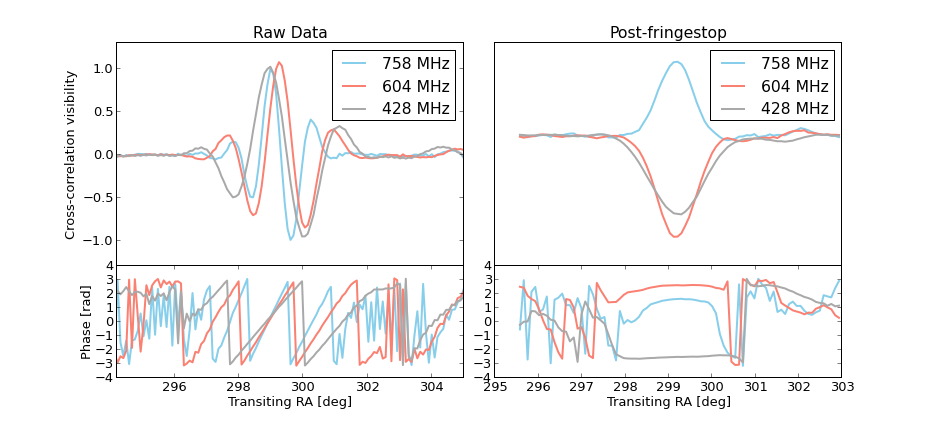
\includegraphics[trim={1in 0in 1in 1in}, width=\smwidth]{./figures/beamforming/thesis_fringestop.png}
\caption[abc]{An example of the fringestopping process that is 
 necessary for gain calibration off of a transiting point-source. Since 
 the phase of a visibility will have a time- and frequency-dependent 
 component, the measured correlation will fringe as the earth rotates in 
 a chromatic way. This effect can be removed by multiplying each visibility by 
 $e^{-i \phi_{m, n}(\rm t, \nu)}$, as determined by Eq.~\ref{eq-fringestop_phase}. 
 The top left panel shows the raw correlation between feeds 1 and 129 as a function of transiting
 $RA$, which are of the same polarization but 
 on opposite cylinders, separated by 21 m. We plot  
 three different frequencies. The panel below the top left
 shows the same complex visibility's phase. The slope, or fringe-rate, decreases 
 at lower frequencies, as expected. The right panel show the same data 
 after running it through the fringestopping pipeline. Though the resulting 
 phases are near flat, implying that the baseline is no long fringeing, 
 the visibilities are not purely real; this is because there are residual 
 instrumental phases. These phases can be solved for using an 
 eigendecomposition now that the array is phased up to a single point-source.}  
\end{center}
\end{figure}

% -------------------------------------------- FIGURE 1 --------------------------------------------


The visibilities we measure can be thought of as 
the upper triangle of an $N\times N$ complex Hermitian 
matrix, $\mathbf{V}$. This is simply the outer product of the 
signal vector, $\mathbf{x}$, with its Hermitian conjugate. 

\begin{align}
\label{eqn-corrmat}
\mathbf{V} = \mathbf{x} \mathbf{x}^\dagger &\approx \begin{pmatrix}
|g_0|^2\, e_0^2 &  & ... & & & \\ 
 &  &  & &  g_n g_m^* e_n e_m^*& \\ 
 &  &  \ddots & & & \\ 
 &  &  &  & & \\
&&&&&&\\
 &  &   &  & &  |g_N|^2 \, e_N^2
\end{pmatrix}
\end{align}
\\

If the sky is composed of a single point-source
then this matrix will be rank one, i.e. there is only one 
non-zero eigenvalue. One can see this by referring to Eq.~\ref{eqn-tsky} 
and noting that if the data has been fringestopped, then the phase 
component (which is different for each correlation) goes away and the 
sky temperature (which is the same) can be factored out of
Eq.~\ref{eqn-corrmat}, which becomes

\begin{equation}
\mathbf{V} = T(\mathbf{\hat{k}_{\textrm{ps}}}) \, \mathbf{g} \mathbf{g}^\dagger.
\end{equation}

\noindent Therefore by diagonalizing the correlation matrix $\mathbf{V}$ 
we get a complex eigenvector corresponding to the largest 
eigenvalue, and that eigenvector is proportional to the gain vector $\mathbf{g}$. 
The phase of this eigenvector will be an estimate for the instrumental 
phases, $\phi_{g_n}$, up to some unknown global offset. The goodness 
of this calibration depends on the validity of our assumption 
that the correlation matrix is rank one. We can estimate the 
error on the calibration solution as the ratio of the second largest 
eigenvalue, $\lambda_2$, to the largest, $\lambda_1$. For typical 
frequencies we get values of $\frac{\lambda_2}{\lambda_1}\sim2\%$ 
when using Cyg A or Cas A.

These algorithms have been implemented in a pre-beamforming 
pipeline written in {\tt Python}. Every day a point-source transit 
is fringestopped and a calibration solution is solved for 
at each frequency.
The source chosen depends on the solar time of its transit: Since the
sun is extraordinarily bright in our band it will be in our side-lobes 
as long as it is above the horizon,
so the transit has to be 
at night for good calibration solutions. Historically, 
we have used Cygnus A in the spring and summer, Cassiopeia A 
in the summer and fall, and Tau A in the winter. 
Whatever we calibrate off of, the phases of that solution are 
written to pickle files that are then fed to the Pathfinder's FPGAs.
The FPGA then applies complex gains after channelization, which 
in theory should provide the beamforming kernel with voltages 
whose phases are purely geometric. 

\subsection{First coherent light}
Although the majority of the back-end was written within a couple  
of months, the beamformer required substantial 
on-sky testing and subsequent debugging. One important debugging tool 
came from utilizing the equivalence of the summed-and-squared
high-cadence data that was produced by the beamformer with the 
full-$N^2$ integrated data. This is true because the correlation 
step does not erase any fundamental information about the electric field. 
The latter is nominally taken with $\sim21$ second
time samples for 32,896 correlation products coming from 256 feeds. 
The former is a sum over the feeds which can be integrated in time 
arbitrarily after squaring. Ignoring the time rebinning for a moment,
we can write the squared formed beam as,

\begin{align}
X_{\rm BF} X_{\rm BF}^* &= (w_1 x_1 + w_2 x_2 + ... + w_N x_N) (w_1 x_1 + w_2 x_2 + ... + w_N x_N)^*\\
&= |w_1|^2|x_1|^2 + ... + |w_N|^2|x_N|^2 + ... + w_1 w_2^* x_1 x_2^* + w_2 w_1^* x_2 x_1^* + ... , 
\end{align}

\noindent where, as before, $w_n$ are the 
complex weights applied in the beamformer 
and $x_n$ is a voltage stream from antenna $n$.
This can be rewritten as the sum of the 
auto correlations and twice the real part of the recorded 
phase-shifted cross-correlations.
\\

\begin{equation}
\label{eqn-bf_sum}
X_{\rm BF} X_{\rm BF}^* = \sum_{n\le N} |w_n|^2 V_{n, n} + 
2 \sum_{\substack{n,m\le N \\ n<m}} \Re e\{W_{n, m} V_{n, m}\}
\end{equation}
\\

In this equation we have let $W_{n, m} \equiv w_n w_m^*$.
Since the correlation matrix is Hermitian, its top 
and bottom triangles are redundant and one needs only to 
record $\frac{1}{2} N (N+1)$ of the $N^2$ pairwise products.
If we wrote all pairwise correlations, we would simply need 
to sum the correlation matrix after applying the relevant 
weights, i.e. summing after the Hadamard
product, $\mathbf{W} \circ \mathbf{V}$. This is identical 
to Eq.~\ref{eqn-bf_sum} if both matrices are Hermitian. 

Using the equivalence we have just described, one can compare the 
output of the beamformer to 
the $N^2$ visibilities after applying complex 
weights and summing the correlations. This is effectively 
off-line beamforming, though the cadence is too slow for 
the science goals of the real beamforming 
back-end, namely studying the time-variable sky. 
As a first test, 
we would form a stationary beam with only two feeds and let a 
bright point-source like Cas A drift through, 
producing a fringe pattern. We would then take 
the corresponding Cas A transit from the correlated ``cosmology" 
acquisition, using Eq.~\ref{eqn-bf_sum} and giving only non-zero 
weights to the two relevant feeds, and check if the two
fringe patterns were identical. We carried out a series 
of tests of escalating complexity, for example including more feeds in the sum, updating 
phases in real-time in order to track sources, and deliberately 
switching the weights with their conjugate to see if the fringe 
direction changed. Through these tests several bugs were discovered, 
including spherical trigonometry errors in the phase 
calculations and a disagreement between one piece of code's 
definition of $LST$. 

The final hurdle was more fundamental to CHIME's architecture,
though in principle it should not affect the cosmology experiment. 
It was found through 
early pulsar observations that the beamformer was only summing
coherently when the instrumental phases that are removed in 
the FPGAs are solved for with the lower-triangle of the correlation 
matrix. In other words, instrumental phases were not properly 
removed in the correlator unless they were applied as 
$e^{+i\phi_{g_n}}$ instead of $e^{-i\phi_{g_n}}$, as one would expect.
The perplexing thing was that in two years of analyzing 
the visibilities output by the correlator, nobody noticed a 
error in the sign-convention. And indeed, when we started to look
at the phase of the raw visibilities, we found the argument 
of an east-west baseline increases with time, which is 
what one expects from an upper-triangle correlator. This 
apparent paradox was solved by discovering \textit{two} sign 
reversals, one in the F-engine and one in the X-engine, that
effectively cancel each other out, but only if both are applied. 

Our digitizers sample at 800 MHz, taking advantage of the observing 
band between 400-800 MHz being in the second Nyquist zone.
However, when we channelize
the incoming time-stream data in the FPGAs, the complex conjugation 
associated with the aliased second Nyquist zone was not considered during the 
Fourier transform. Therefore the channelized voltages leave the F-engine 
with an opposite sign in the exponential. When they are correlated
in the X-engine it is also done in reverse order as, 

\begin{equation}
V_{n, m} = x_n^* x_m,
\end{equation}

\noindent as opposed to the upper-triangle correlation described by 
\citet{2015arXiv150306203K}, 

\begin{equation}
V_{n, m} = x_n x_m^*.
\end{equation}

The second sign convention error does not affect the beamformed 
output, since that data stream is never correlated. We therefore 
needed to account for this for the back-end to work. An example 
of an early verification of the beamformer's sign convention 
and the first successful tracking observation is shown in Fig.~\ref{fig-bf_b0329}. 
The collaboration has decided to keep these sign conventions as is
and make note of it going forward, rather than re-write any low-level 
software.


\begin{figure}[!h]
\label{fig-bf_b0329}
\begin{center}
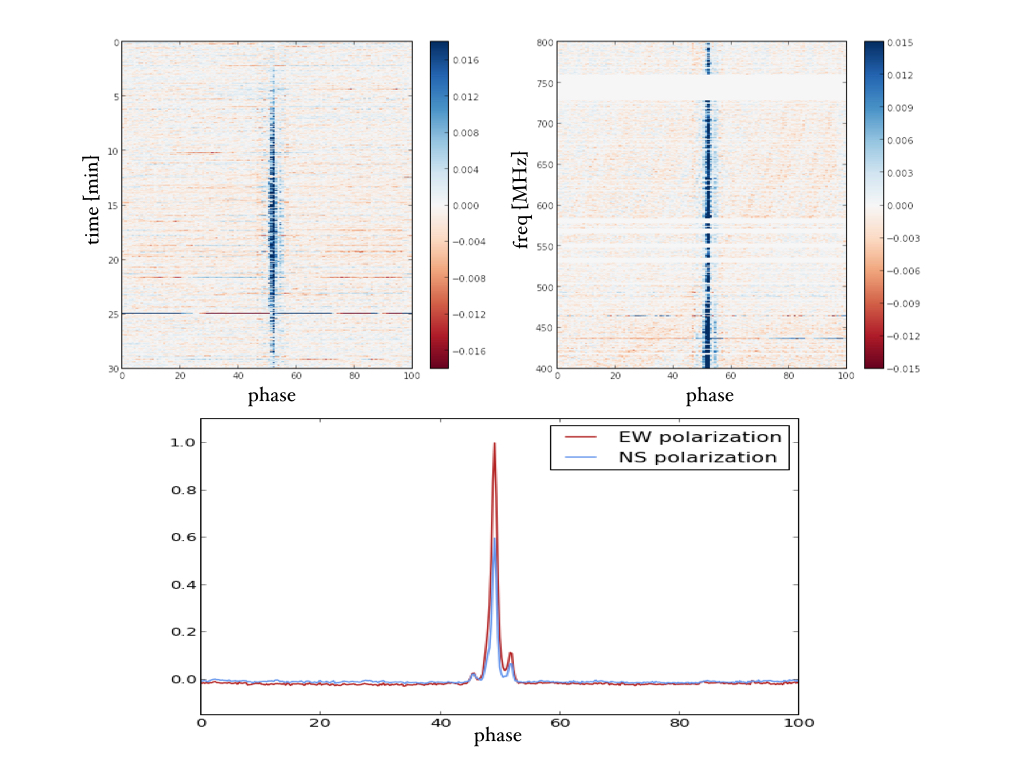
\includegraphics[trim={0.8in, 0in, 0in, 0in}, scale=0.5]{./figures/beamforming/b0329_testing.jpeg}
%\vspace{0.0cm}
\caption[abc]{First coherent pulsar observations with CHIME. This 
brief observation of B0329+54 provided us with an idea 
of the instrument's sensitivity and polarization response. 
Perhaps more significantly, it taught us that 
that our X-engine is a lower-triangle correlator, rather than 
upper-triangle like we thought, and that our F-engine \textit{also}
conjugates with the opposite sign. \textit{top left:} waterfall plot
of the pulsar's Stokes I profile over the $\sim$30 minutes when the 
source enters then exits our beam. \textit{top right:} frequency 
vs. phase Stokes I, integrated over roughly 15 minutes. 
\textit{bottom:} time- and frequency-averaged pulse profile 
for the two polarizations autocorrelations. The difference between 
the east-west and north-south beams give an estimate for Stokes Q, which 
includes both intrinsic polarization ($\sim10\%$ for this source)
and instrumental leakage.} 
\vspace{0.4cm}   
\end{center}
\end{figure}


\section{FRB VLBI search}
\label{vlbi_frb}

In 1967 Canada achieved an historic feat by doing 
the first ever successful very long 
baseline interferometry (VLBI) observation. The fringes were 
obtained between DRAO and ARO, with a baseline of 3,074\,km 
\citep{1967Natur.215...38B}. 
This result was given a ``Milestone'' award from 
The Institute of Electrical and Electronics Engineers (IEEE), 
which was also awarded for the inception of the Internet, transmission 
of transatlantic radio signals, and the discovery of Maxwell's 
equations\footnote{http://ethw.org/Milestones:List\_of\_IEEE\_Milestones}. 
We have attempted to recreate the same VLBI baseline, but instead of 
using the considerable spatial resolution on quasars as in 1967, 
we are attempting to localize FRBs, and in place of the 
26\,m telescope we will use the Pathfinder's formed beam.


\subsection{Motivation}

The CHIME Pathfinder is meant to have only one synthetic beam. 
Its purpose is primarily to act as a test-bed for the more powerful 
pulsar and FRB back-ends that will be attached to the 
full four-cylinder CHIME. However since the Pathfinder is on 
sky at all times and the beamformer we have built does not 
interrupt the ongoing cosmology acquisition, we decided to 
build a preliminary FRB search. We also have as many as three 
other telescopes onto which we can mount 
CHIME feeds and observe in our band: the Algonquin Radio Observatory (ARO), 
the John A. Galt 26m, and the Green Bank 140ft telescope. This would
allow for the first ever VLBI detection of an FRB. 

This is interesting for a few reasons. From a development 
standpoint it allows us to understand better various stages of the 
CHIME-FRB pipeline, including the rate of 
RFI false-positives, our algorithm's search 
efficiency, and specs on the regularity and precision of instrumental 
gain removal. It will also give us a good sense of how the real CHIME 
beams behave on the sky. 

Beyond just instrumental development, this work
opens up several avenues for new science. 
Most interestingly, 
we could reasonably expect to see a few bursts per year in 
VLBI. Localization is by far the most 
important next step in determining the origin of FRBs, and 
such a long-baseline detection would achieve this. This particular VLBI 
array, whose baselines are thousands of kilometers, would provide 
the necessary spatial resolution to locate the source 
within its galaxy. This is demonstrated in Fig.~\ref{fig-m51}.
On top of this, we would not only detect a burst with 
milli-arcsecond resolution, but it would also be the first source 
in our band, at 400-800 MHz. We 
would be writing baseband and therefore full-polarization information,
which is not true of most FRBs.

\begin{figure}[!h]
\label{fig-m51}
\begin{center}
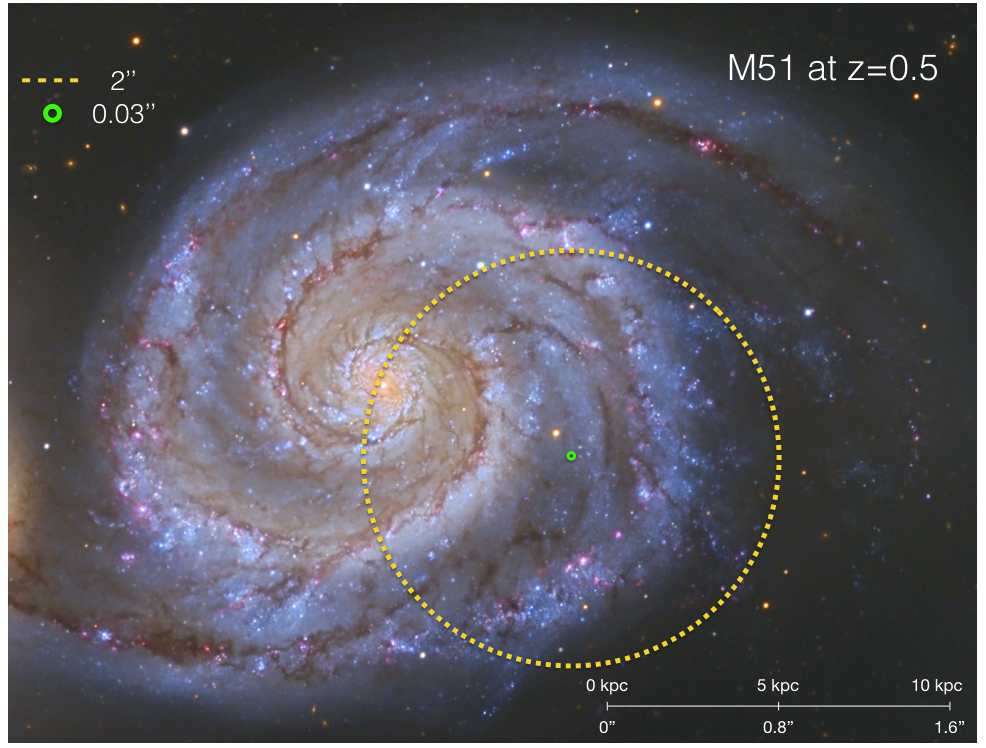
\includegraphics[trim={0in, 0in, 0in, 0in}, width=\textwidth]{./figures/beamforming/m51green.jpeg}
\caption[abc]{A visual demonstration of the difference between 
     30 milli-arcsecond resolution and an $\sim$arcsecond beam.
     This shows the need for extremely long baselines 
     in a FRB VLBI effort.
     The image shows M51, which is about 20 kpc across, if it
     were at redshift 0.5. 2" resolution ($\sim$10$^5$ wavelengths, or $\sim$
     50\,km at 600 MHz.) cannot distinguish between the 
     Galactic center and the edge of the disk. On the other hand,
     0.03" ($\sim$10$^7$ wavelengths)
     is the resolution of the 3,074\,km DRAO-ARO baseline,  
     which can localize the source well within the galaxy, even at 
     high redshifts.}  
\end{center}
\end{figure}

The Pathfinder beam could be used on its own to constrain 
the location of FRBs via their brightness distribution.
Specifically, we could test the claims made by
\citet{2016arXiv160606795V} who suggest there is now evidence 
for a flat fluence distribution of FRBs, implying 
that they are cosmological in nature 
(see Chapter \ref{chapter:frb_statistics} for our detailed statistical
analysis of this issue). 
This would mean there are a relatively large number of 
ultra-bright bursts, 
and that survey speed is determined by FoV rather than 
thermal sensitivity. The Pathfinder would be an excellent 
tool to test this hypothesis, as a non-detection after multiple months 
would call it into question. 


\subsection{Implementation}

We have had a working beamforming back-end on the CHIME 
Pathfinder since October 2015. 
A beamforming kernel in the GPUs sends data over two 10 GBe
lines to an acquisition node, {\tt moose}, 
in the VLBI Data Interchange Format (VDIF) 
specification\footnote{http://www.vlbi.org/vdif/docs/VDIF\_specification\_Release\_1.1.1.pdf}. 
The back-end has been used primarily 
for short tracking pulsar observations, but had stability issues 
on timescales of $\sim$days, meaning we could not run it 
for long periods without interfering with the regular cosmology acquisition. 
However in the past several months a number of new features 
were added that allow not only long-term beamforming captures, 
but also transient searching. 
 
A real-time, multithreaded acquisition code that takes in the VDIF 
packets coming out of the X-engine, and rearranges them to either be written to disk or search for 
FRBs\footnote{https://github.com/kmsmith137/ch\_vdif\_assembler}. Attached 
to this packet reader was a tree-dedispersion search code, some of 
which had been used before on Green Bank 100\,m data and a real-time ARO 
search\footnote{https://github.com/kiyo-masui/burst\_search}.
The CHIME acquisition software {\tt kotekan} was 
altered in a number of ways, fixing the long-term 
stability issues in the beamforming kernel. These systems 
were synthesized into a real-time transient search back-end 
that has been on sky since May 2016. 
It is outlined in Fig.~\ref{fig-bf_diagram}
on page \pageref{fig-bf_diagram}. 


\begin{figure}[!h]
\label{fig-bf_diagram}
\begin{center}
\vspace{-0.5in}
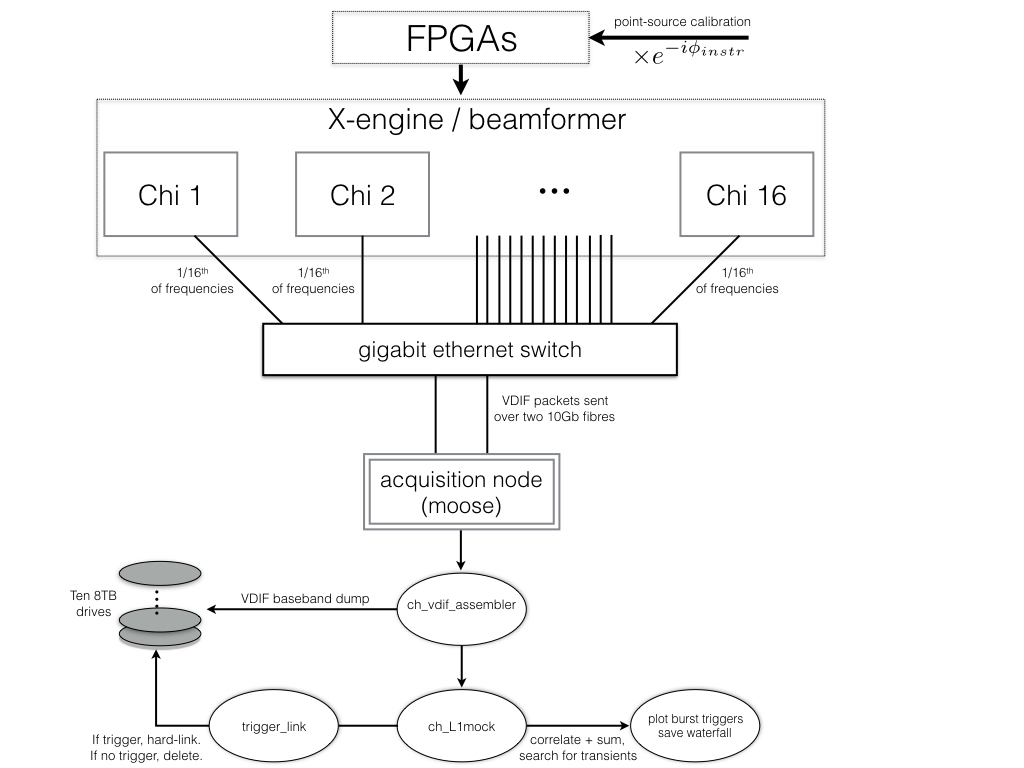
\includegraphics[trim={1.in, 0in, 2.5in, 0in}, width=1\textwidth]{./figures/beamforming/moose_diagram.png} 
%\vspace{0.0cm}
\caption[abc]{Block diagram of the beamforming back-end on CHIME Pathfinder. 
A calibration solution is obtained from a bright point-source transit, 
the phases of which are fed into the FPGAs where they are applied as a 
digital gain. All antenna signals are then sent the $X$-engine, 
comprised of 16 GPU nodes. Each node applies geometric phases then 
sums the voltage stream across all antennas with the same polarization. 
The two resultant beams are then sent to our acquisition machine {\tt moose} 
as {\tt VDIF} packets, where a multi-threaded capture code, {\tt ch\_vdif\_assembler}. 
At this point the baseband data are either written to disk as scrambled baseband 
{\tt VDIF}, or they are reorganized in time and frequency. The ordered data are 
searched for FRBs after squaring and integrating to $\sim$millisecond cadence 
using a tree-dedispersion algorithm. If there is a trigger, then the corresponding 
baseband data is hard-linked. Old files that haven't been hard-linked are deleted
periodically.}
\end{center}
\end{figure}

Since CHIME is a transit telescope with a long north-south beam, 
our formed beam is effectively confined to the meridian. This means
we must choose an optimal declination on which 
to park the beam. As a sanity check, we have spent roughly 
half the time pointed 
at the declination of pulsar B0329+54, which is the 
brightest switching source in the northern sky in our band. It 
is dispersed with 26.833 pc cm$^{-3}$ and its individual 
pulses are bright enough to detect, meaning our tree-dedispersion 
algorithm ought to find its individual pulses. The search 
algorithm looks at time blocks of 100 seconds, searches 
for DMs between 10-2000 pc cm$^{-3}$ with widths between 
1-100 ms, and looks for peaks above 8$\sigma$. If it finds something
it ``triggers'' and writes out an image file containing the peak 
in DM / arrival time space, a dedispersed waterfall plot, a dedispersed 
pulse profile, and a fluence frequency spectrum. An example 
of the B0329+54 trigger output is shown in Fig.\ref{fig-b0329_trigger}. 
It also writes {\tt numpy} arrays containing the squared and summed 
intensity data. It then moves on to the next block of 100 seconds, 
overlapping with the previous one by 18 seconds. 


\begin{figure}[!h]
\label{fig-b0329_trigger}
\begin{center}
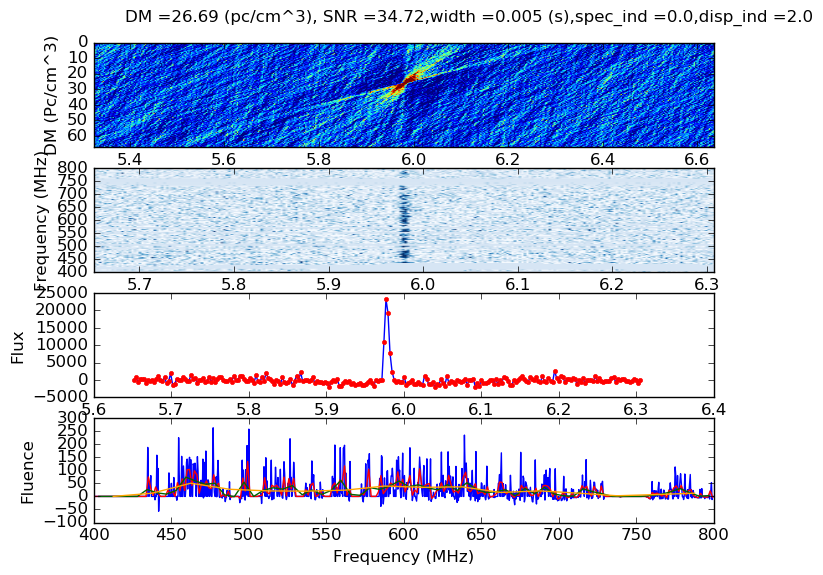
\includegraphics[trim={0in, 0in, 0in, 0in}, scale=0.75]{./figures/beamforming/b0329_trigger.png}
\caption[abc]{Example of a figure created after a trigger 
on the Pathfinder FRB search. This trigger was during the transit of 
pulsar B0329+54, on whose declination our synthetic beam was 
parked. Further information about the pulse is 
included at the top of the figure, including 
signal-to-noise ratio, width, and dispersion index. Though the 
beam is not well calibrated in absolute flux, this pulsar 
is of order 10 Jy, so this pulse might be half as bright 
as the original Lorimer burst \citep{lorimer-2007}. 
\textit{Top panel:} The search results 
in dispersion measure vs. arrival time space. The red, butterfly-like 
cluster of points around DM of 25 pc cm$^{-3}$ and arrival time 
6 seconds into the 100 second block, 
shows the detection of a single B0329+54 pulse. 
\textit{Second panel:} A frequency 
vs. time colour map showing the dedispersed pulse. \textit{Third panel:} 
Pulse profile for this trigger, averaged over frequency after 
masking RFI and weighting by inverse system temperature. \textit{Bottom panel:}
Fluence vs. frequency plot of the pulse.}  
\vspace{0.4cm}   
\end{center}
\end{figure}

\subsection{ARO FRB search}

At ARO we have implemented a similar back-end to the 
one operating at DRAO. Luckily, the computing 
requirements are less demanding. Since there is only 
one dual-polarization feed mounted on the dish, 
we need only one FGPA board and one processing node. 
At DRAO 1/16$^{\textrm{th}}$ of frequencies are 
handled by each GPU node, which means they arrive scrambled
at the acquisition machine, {\tt moose} (see ~\ref{fig-bf_diagram}). 
Software had to be written to re-order in time and frequency 
data in real-time. At ARO, all 1024 frequencies arrive in contiguous 
blocks at each frame, meaning we simply listen to a socket 
for the packets, square and sum, then search for FRBs. The ARO 
back-end is outlined in Fig.~\ref{fig-aro_diagram}.


\begin{figure}[!h]
\label{fig-aro_diagram}
\begin{center}
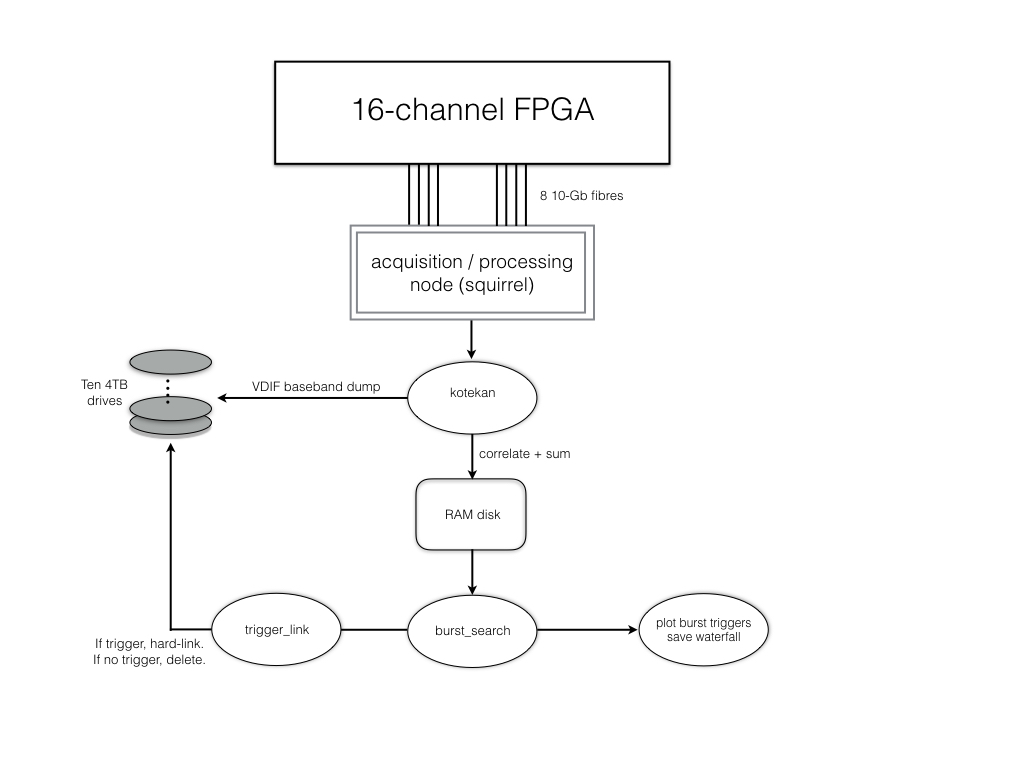
\includegraphics[trim={0in, 0in, 0in, 0in}, width=\textwidth]{./figures/beamforming/aro_diagram.jpeg}
\caption[abc]{This figure shows a block diagram of the basic 
     FRB search setup at ARO. A single 16-channel FPGA
     channelizes the 800 Ms/s data and sends 1024 frequencies 
     to an acquisition node, {\tt squirrel}, at a cadence of 2.56 $\mu$s.
     Those data are squared, summed, and dumped to a RAM disk, 
     where it is searched for FRBs between 10-2000 pc cm$^{-3}$.}
\vspace{0.4cm}   
\end{center}
\end{figure}

\subsection{Results}

\subsection{A flat brightness distribution?}
As we discuss in chapter \ref{chapter:frb_statistics}, there is 
a large uncertainty in the FRB rate between 400-800 MHz. There 
is even greater uncertainty in the expected rate for a 
telescope like the CHIME Pathfinder. This is because at this time
all FRBs
have been detected with large collecting area, highly sensitive single-dish 
telescopes (GBT, Parkes, and Arecibo). Therefore in order to 
extrapolate the rate estimates on to the Pathfinder, which 
does not have much collecting area and whose beam is quite large, one 
needs to know the underlying flux distribution. As we will show 
in Chapter \ref{chapter:frb_statistics}, the rate depends on the product 
of the telescope's field-of-view (FoV) and a thermal sensitivity term. 
For a single-feed receiver, the FoV is given by 
$\sim \left(\frac{\lambda}{D}\right)^2$, which scales inversely with 
collecting area, $A$. The thermal component depends linearly
on forward gain and therefore collecting area. Combining these, 
the rate is, 
\begin{align}
r_o &= \textrm{FoV} \times \left(\textrm{sensitivity}\right)^\alpha\\
     & \propto A^{-1} A^\alpha,
\end{align}
where $\alpha$ is the FRB flux distribution's power-law index, which is 
$3/2$ if FRBs are non-cosmological and Euclidean. If $\alpha < 1$, 
as is expected in the cosmological FRB scenario, then 
small telescopes are actually advantageous over large single-pixel telescopes 
since the beamsize becomes more important when $\alpha-1$ is negative. 

With a dish like the Pathfinder
we expect the rate to be 
roughly 10 times higher if $\alpha\approx 0.8$ (cosmological scenario) 
compared to the Euclidean scenario. This is because its relatively 
low sensitivity per steradian requires there be large numbers 
of very bright bursts, which one gets from a flat distribution.

During the search 
millisecond intensities can be written to disk.  
We can therefore look for slow pulsars 
and RRATS, since a significant fraction of the Galaxy transits each day.
\subsection{False positives}

Most transient searches are plagued by non-celestial sources masquerading 
as astronomical events. 
In the case of DM searches on 
radio telescopes, these can be caused by RFI, numerical relics 
in the signal chain, or statistical fluctuations. 
At UTMOST, \citet{2016MNRAS.458..718C} found 
10$^2$ events per hour in transit mode across all beams. \citet{2015MNRAS.451.3933P}
found the source of an elusive but persistent set of triggers 
to be due to an on-site microwave oven's magnetron shutdown phase. These 
``Perytons" are unique in their conspiratorial ability to 
look like a real burst, but they are a subset of a broader zoo 
of RFI-induced false triggers. 

At DRAO, although the region is officially 
protected from radio contamination, about 15$\%$ of the CHIME
band is presently lost to RFI (see the bottom left 
panel of Fig.~\ref{fig-lte_trigger}). Recently, Rogers Communications 
paid several billion Canadian dollars for a 700 MHz 
Long-Term Evolution (LTE) band for cellphone service.
Unlike the satellite television stations that we see at 500-600 MHz, 
the LTE band fluctuates on timescales of milliseconds to seconds, 
which can affect a millisecond transient search. 
Fig.~\ref{fig-lte_trigger} shows an example of this RFI false 
positive from the LTE band. 


%trim={<left> <lower> <right> <upper>}
\begin{figure}[!h]
\label{fig-lte_trigger}
\begin{center}
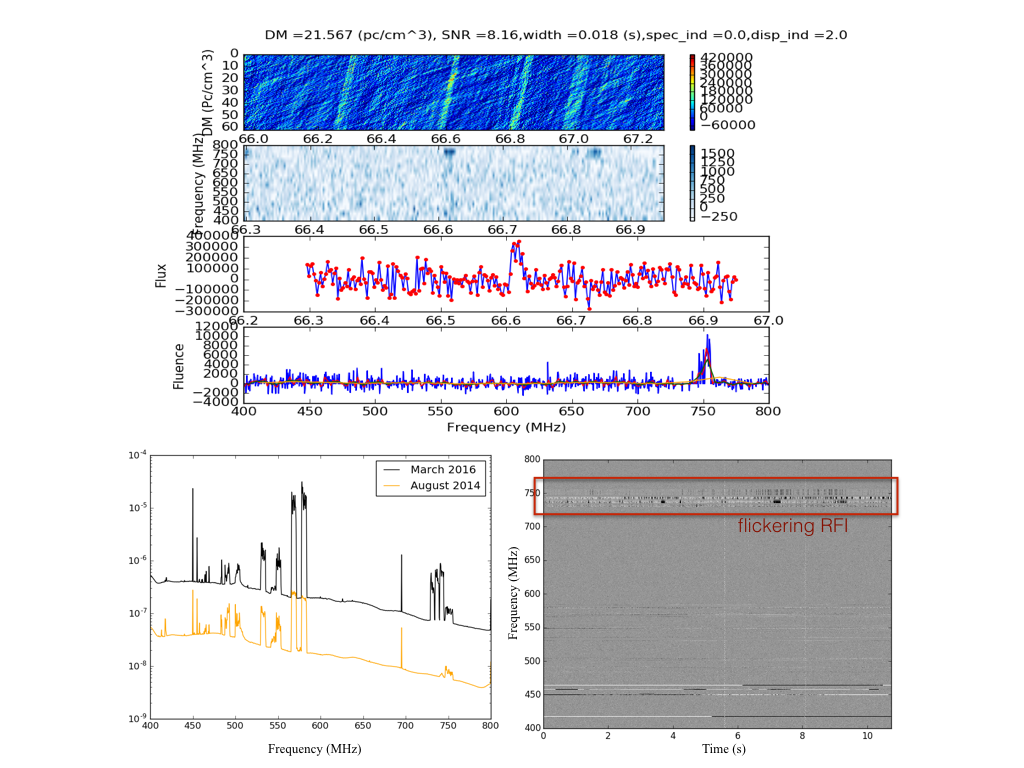
\includegraphics[trim={0in 0in 0in 0in}, scale=0.5]
{./figures/beamforming/lte_trigger.png}
\vspace{0.0cm}
\caption[abc]{A false positive trigger caused by the flickering 
LTE band that, the likes of which 
caused $\sim$90$\%$ of the alerts before it was removed.
It is of course simple to reject; one can just mask 
out the relevant channels.
However, it provides a useful example of the types of 
short-timescale RFI that can affect an FRB survey.}
\end{center}
\end{figure}


To mitigate this, frequency channels that are known 
to be contaminated are masked out. Zeroing the LTE band,
for instance, removed $\sim$90$\%$ of the false-positive triggers. 
Once this was done, we find a false-trigger rate of 
approximately one per two hours. This is estimated 
by inspecting each trigger visually. Though the rate 
had been greatly reduced, it is still a 1000:1 ratio of 
false positives to real events in the case where we detect 
one FRB every three months (for a detailed estimate see Sect.~\ref{chimerate}
in Chapter \ref{chapter:frb_statistics}). With this in mind, 
the SNR threshold was increased from 8$\sigma$ to 9$\sigma$. 
This was done because the false triggers tend to occur 
with significance very close to the cutoff. Even if they are 
not perfectly Gaussian, the number of 6$\sigma$ events is 
far larger than the number of 8$\sigma$ events, of which 
there are many more than 10$\sigma$ events. 

This is less true for FRBs, whose brightness distribution 
are described by a power-law. Using a signal-to-noise 
cutoff of $s_\mathrm{min}$, the fraction 
of detected events one expects above $s$ is given by,

\begin{equation}
f(>s) = \left(\frac{s}{s_\mathrm{min}}\right)^{-\alpha}.
\end{equation}

\noindent The signal-to-noise at which $f=0.5$ is 
12.7 and 19 for $\alpha=1.5$ and $\alpha=0.8$ respectively. 
The fraction of events one expects between 8-9$\sigma$ is 
$f(>8) - f(>9) \approx 16\%$ for the Euclidean case, 
and $8\%$ if $\alpha$ is 0.8. Therefore half the true events 
the experiment detects will unmistakably celestial, whether they 
are cosmological or Euclidean, and by increasing the threshold 
to 9$\sigma$ one only decreases the survey speed by of order 
ten percent. 

\begin{figure}[!h]
\label{fig-scatterhist}
\begin{center}
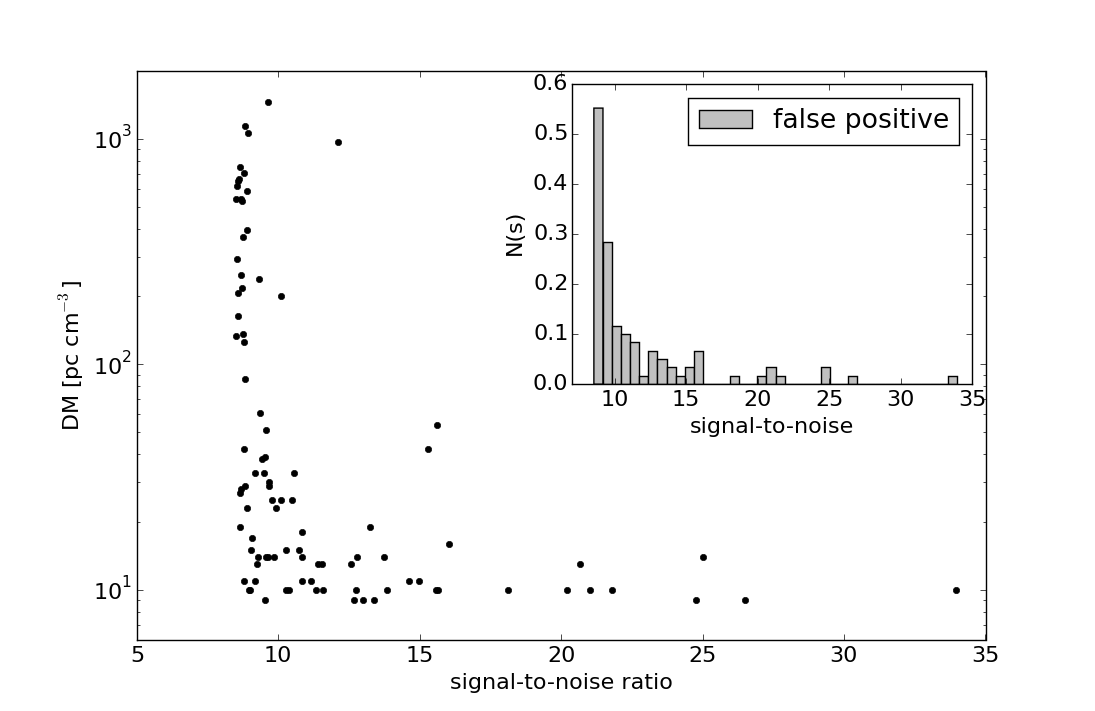
\includegraphics[trim={0in 0in 0in 0in}, scale=0.5]
{./figures/beamforming/dm_dist_falsepositives.png}
\vspace{0.0cm}
\caption[abc]{This figure shows the distribution 
     of false-positives in DM and signal-to-noise. The 
     embedded normalized histogram shows the clustering of events 
     near the threshold of 8$\sigma$. One can see that by 
     increasing the threshold to $\sim$9-10, half of all 
     false triggers could be avoided. The scatter plot shows 
     DM vs. signal-to-noise for the same set of triggers. The 
     high-significance tail in the histogram seem to all be clustered 
     at very low DMs, near the minimum DM that is searched 
     (10 pc cm$^{-3}$). This makes it easy to differentiate truly 
     ``bright" events from high-signal-to-noise false positives.}
\end{center}
\end{figure}

\begin{figure}[!h]
\label{fig-scatterhist}
\begin{center}
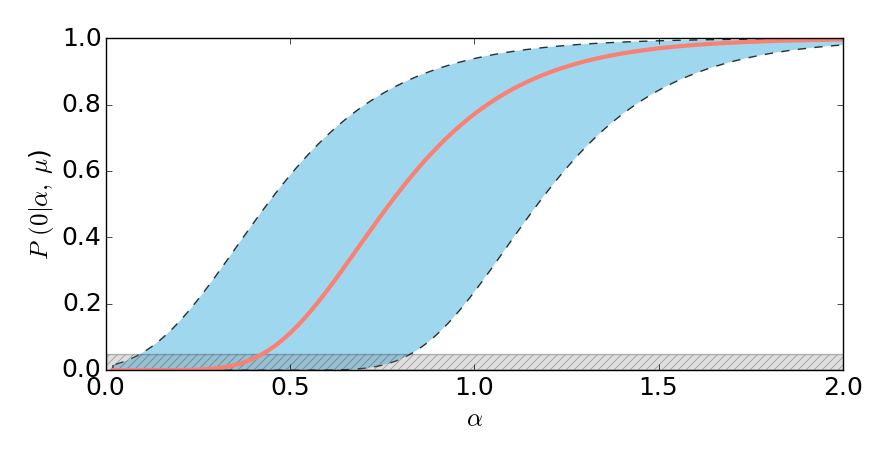
\includegraphics[trim={0in 0in 0in 0in}, scale=0.65]
{./figures/beamforming/alpha_limits.png}
\vspace{0.0cm}
\caption[abc]{Early limits on the flux distribution 
     parameter $\alpha$ from the Pathfinder 
     FRB search. }
\end{center}
\end{figure}

\section{Conclusion}
\label{sec:beamforming_conclusion}

Digital beamforming is a powerful tool that affords modern 
radio telescopes enormous fields-of-view without 
sacrificing resolution. It is no longer strictly necessary 
to build large steerable reflectors, the cost of which scales 
roughly as diameter cubed\footnote{https://www.astron.nl/~mag/dokuwiki/lib/exe/fetch.php?media=radio\_astronomy\_lec\_2\_ma\_garrett.pdf}, 
since spatial filtering can be done in software.
In this chapter 
we have walked through the basic mathematical formalism 
for beamforming. We have calculated the requisite geometric 
delays, which also allow us to ``fringestop" the data. 
This process was 
put to use for phase-calibration of transiting point-sources, 
a step which is vital to beamforming. 

The CHIME Pathfinder now has a stable beamforming back-end
that runs in parallel with the full-$N^2$ cosmology acquisition.
The back-end provides us with a tracking synthetic beam that 
dumps baseband data to disk with 1024 391 kHz channels at 
2.56 microseconds. We have outlined the commissioning of this 
back-end, including the first coherent pulsar observations on CHIME.

We have also described a new project to localize FRBs with 
milli-arcsecond resolution using VLBI between Penticton, BC 
and Algonquin Park, Ontario. The first component 
of this project is a real-time transient search on the Pathfinder's 
formed beam, which has been on-sky searching since early May 2016. 
Though we have not found any FRBs yet, the non-detection 
allows us to test the cosmological-origin hypothesis. This is 
because FRBs coming from $z\approx0.3-1$ will have a flatter 
flux distribution than a more local population, which 
will obey $N(>S)\propto S^{-1.5}$. The cosmological hypothesis implies that 
there exists surplus of ultra-bright bursts that could be 
seen by a relatively insensitive instrument like that Pathfinder.
We found that with 

The ARO 


% ================================================================================
% ACKNOWLEDGEMENTS
% ================================================================================


  

%\include{./sections/frb_modelling}
%\include{./sections/frb_statistics}
%\chapter{Pulse Microstructure}
\label{chapter:microstructure}
\chaptermark{Microstructure}

% \textbf{Think this is the largest set of B0329+54 single pulses 
% studied at $\mu$s. Check. \\ 
% Maybe include gamma arguments P/tms about 1000 for this pulsar 
% seems to be too big for flux tubes \\ 
% bartel \citep{1981A&A....93...85B} observed with 2.5 $\mu s$}

% ================================================================================
% CHAPTER OVERVIEW
% ================================================================================

\section{Chapter Overview}
In this chapter we present results from full-polarization  
single-pulse observations of pulsar B0329+54. 
We have over $10^4$ pulses 
collected with the Algonquin Radio Observatory 46\,m telescope
with 2.56\,$\mu$s time resolution and 390\,kHz 
frequency bins. 
We find microstructure to be a generic broad-band property of 
individual pulses at 400-800\,MHz.
We also analyze B0329+54's quasi-periodic structure
using a reduced autocorrelation function (rACF). 
Unlike in other pulsars, 
we do not find a characteristic timescale in its quasi-periodicity, 
although the range of of periods is consistent with the known
$t_{\mu} \approx 6 \times 10^{-4} P$ and 
$T_{\mu} \approx 10^{-3} P$ relations. 
Our polarimetry results agree with 
\citet{2015ApJ...806..236M}, in that the periodicity 
of both linear and circular polarization microstructure 
traces closely the total power. 
% This is difficult to 
% accommodate in the model where microbursts represent 
% single charge bunches emitting curvature radiation 
% in vacua. 
We also investigate the spectral properties 
of micropulses within a sub-pulse. It is shown that the microstructure not 
only has a wide bandwidth, but that adjacent broad-band 
microstructures can have very different spectra. 

%================================================================================
% INTRODUCTION
% ================================================================================

\section{Introduction}

Within only a few years of the discovery of pulsar B1919+21
in 1967 it had 
become clear that there was great variation between 
individual pulses, and 
even structure within pulses 
\citep{1968Natur.218.1122C, 1975ApJ...196...83M, 1975Natur.257..293R}. 
% Insert citation for this variation.
Each pulsar's folded and integrated profile 
is highly reproducible and specific to that pulsar, 
however the pulses of which they are comprised are 
diverse in a multitude of ways \citep{1998pulsarastronomy}. 
Variation of polarization fraction and mode, intensity 
fluctuations of sub-pulses, and variable arrival times 
are examples of the pulse-to-pulse dynamics. Nulling 
and pulse drifting are also common, and still these 
ostensibly stochastic phenomena result in recognizable 
folded profiles. An example of this is shown in 
Fig.~\ref{fig-pulse_outline}, in data taken at ARO. 

\begin{figure}[!h]
\begin{center}
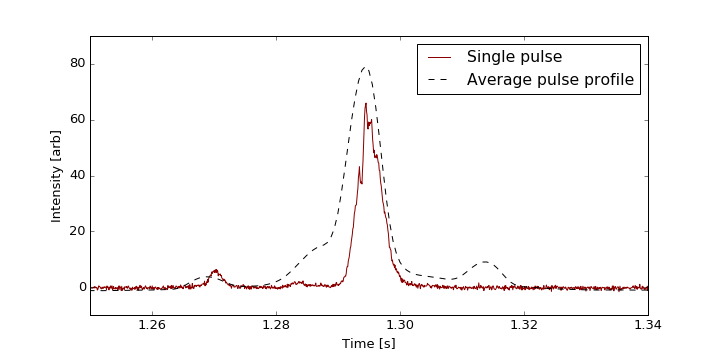
\includegraphics[trim={0in 0in 0in 0in}, width=1\textwidth]{./figures/microstructure/B0329_average_single.png}
\vspace{0.0cm}
\caption{The average profile of pulsar B0329+54 (dashed, black line)
plotted over a single pulse (solid, maroon line). Though 
there is significant variation from pulse to pulse in 
each of the sub-components (of which there are 
as many as 9 \citep{2001ApJ...555...31G}), 
the average profile is 
well known and repeatable. It can be thought of as a 
probability distribution from which the power in each 
phase bin for a single pulse is drawn.}  
\vspace{-0.4cm}   
\label{fig-pulse_outline}
\end{center}
\end{figure}

Understanding the physical mechanism by which pulsars emit in the 
radio has proven one of the hardest problems 
in modern astrophysics \citep{1975ARA&A..13..511G, 2000ASPC..202..721M}. 
Most of what is known has come 
from folded pulse profiles, but given the substantial 
phenomenology on timescales of individual pulses, there 
is good reason to study them.

On the shortest timescales, microstructure appears in a number of pulsars 
\citep{1975PhDT.........9C, 1982ApJ...254L..35B, 
1998A&A...332..111L, 2002A&A...396..171P}. 
This usually involves 
intensity variation on sub-millisecond timescales. 
They can exhibit periodic oscillatory fluctuations 
as well as broad-band features \citep{1981A&A....93...85B}. 
%\textbf{DESCRIBE IN MORE DETAIL}
Although the phenomenon has been seen in a number of slow pulsars 
at a range of frequencies, there is 
no agreed upon explanation for the origin of microstructure 
\citep{1998A&A...332..111L}. 
\citet{vanhorn} argued the phenomenon was not magnetospheric
but rather a result of neutron star vibrations, 
hence the periodic nature of the substructure. 
Another explanation has been to evoke propagation 
effects in the pulsar magnetosphere. Most commonly, though, 
models for these $\sim$microsecond intensity 
fluctuations have assumed it is fundamentally 
related to the emission mechanism 
rather than a separate process occurring elsewhere 
in the magnetosphere \citep{1998A&A...332..111L}.

Before linking microstructure to broader emission mechanisms, 
it is useful to remind ourselves about the potential 
sources of radio emission in pulsars. 
One prominent explanation is the vacuum curvature 
radiation model. Curvature radiation is similar to 
synchrotron except with a pitch angle that is nearly zero.
In the pulsar magnetosphere, this happens when electrons or positrons 
travel along the very strong curved
magnetic field lines, radiating 
at some critical frequency $\nu_c \sim \gamma^3 c/r_B$, 
where $r_B$ is the radius of curvature of the field lines and 
$\gamma$ is the Lorentz factor
\citep{1998pulsarastronomy}. Given the 
expected relativistic electron-positron plasma over-density at the
pulsar's polar caps and the strong magnetic fields there, 
curvature radiation seems like a natural explanation 
for radio emission. One difficulty with the model is that 
due to the exceedingly high brightness temperatures of 
pulsars, it has always been known that 
coherent emission is needed. For the vacuum curvature 
scenario, this requires ``charged bunches" of electrons 
($\sim$10$^{15}$ particles) emitting coherent curvature radiation 
\citep{2004ApJ...600..872G}, and it is not obvious 
how these bunches would be created.

The single-particle vacuum curvature-radiation model 
can be informed by observations microstructure and 
its polarization. Since the sub-pulses that make 
up individual pulses can be further broken down into 
microstructures, those microbursts should show phenomena 
predicted by thoery. The consequences of 
an incoherent sum of charged bunches 
emitting coherent curvature radiation can be found 
in \citet{1990A&A...234..269G} and summarized 
in \citet{2015ApJ...806..236M}.

Few detailed polarization studies of 
microstructure have been carried out. 
\citet{1978A&A....64...27F} commented on the qualitative 
polarization properties of microstructure seen in B1133+16. 
\citet{2002MNRAS.334..523K} quantitatively analyzed polarimetry 
observations of Vela's microstructure. Recently, however, 
\citet{2015ApJ...806..236M} made a convincing case for 
studying short-timescale 
fluctuations of polarized pulsar emission. 
They observed almost three 
dozen sources with $\sim$60\,$\mu$s time-resolution at 
Arecibo with periods ranging from 0.15-3.7 seconds.



% ================================================================================
% THEORY AND IMPLEMENTATION
% ================================================================================

\section{B0329+54 Individual Pulses}

\subsection{Observations}

The data for our B0329+54 single-pulse analysis 
were taken at the Algonquin Radio Observatory (ARO). 
The refurbished 46\,m antenna was mounted with a 400-800\,MHz 
CHIME four-leaf clover feed, the details 
of which are described in Chapter \ref{chapter:chime}. 
We attached to it a custom back-end 
made from CHIME hardware and software that can write voltage 
data to disk with $\sim$390\,kHz spectral resolution 
and 2.56\,$\mu$s temporal resolution. We refer to this as ``baseband". 
Though the data is channelized with a polyphase filter bank (PFB),
the process is invertible and we are able to 
de-channelize in order to coherently dedisperse offline. Data are written 
in the VDIF specification, similar to the Pathfinder data format 
described in Chapter \ref{chapter:beamforming}. However in 
the case of ARO, since we have 2 channels instead of 256, we do 
not need 16 FPGA boards and 16 GPU nodes to process the data. 
Therefore frequencies need not be reassembled because 
each frame contains all 1024 contiguous frequencies. There 
are also slight changes to the header. 
We observed the pulsar for roughly 2 hours on 1 August 
2014, for more than 10$^4$ pulses. 


\subsection{Data post-processing}
\label{sec-b0329analysis}

We use a VLBI pulsar analysis code-base called 
{\tt scintellometry}, which was built for 
correlating baseband data from different telescopes 
with differing data formats\footnote{https://github.com/mhvk/scintellometry}. 
Though the code is able to coherently dedisperse, 
B0329+54 is slow and has a DM of only 
$\sim$27 pc cm$^{-3}$, and we have found it is sufficient to do ``by-channel" 
dedispersion. This means stepping through each frequency 
of the channelized voltage data, inverse Fourier transforming 
that frequency's time series, and dedispersing that up-channelized 
chunk. The resultant DM-smearing in the case of 
B0329+54 is negligible. 

The two dedispersed voltage time-streams are then correlated, 
providing four real numbers per time and frequency. 
Out of these correlations the Stokes parameters 
can be constructed. The four numbers are an autocorrelation for each 
polarization, and the real and imaginary components of the
cross-correlation. The output array is therefore,

\begin{equation}
D = \begin{pmatrix}
\left< X_0X_0^*\right> & \left< \Re e\{X_0X_1^*\}\right >\\ 
 \left< \Im m\{X_0X_1^*\}\right > & \left< X_1X_1^*\right>
\end{pmatrix}.
\end{equation}
\\
\noindent By rearranging these, the Stokes parameters can 
be obtained as follows,
\\
\begin{equation}
\begin{pmatrix}
\left< X_0X_0^*\right> & \left< X_0X_1^*\right >\\ 
 \left< X_0^*X_1 \right > & \left< X_1X_1^*\right>
\end{pmatrix} = 
\begin{pmatrix}
I + Q & U + iV\\ 
U -iV & I - Q
\end{pmatrix}.
\end{equation}


\noindent These intensities are either folded 
or written to a dedispersed time and frequency {\tt numpy} 
array with arbitrary time rebinning. 

Before the polarization data can be analyzed, 
we must remove two effects. The first is the 
sinusoidal phase in frequency introduced by cable delays. 
This comes from that fact that the two polarizations signals, 
$X_0$ and $X_1$, end up with slightly different instrumental 
phases due to things like disparate cable lengths. When 
the signals are correlated, a constant phase offset (time lag) 
becomes a sinusoidal oscillation in frequency. 
Written in terms of the Stokes parameters
this transformation takes,

\begin{equation}
X_0 X_1^* = U + iV,
\end{equation}

\noindent and makes the cross-pol correlation

\begin{equation}
X_0 X_1^* \rightarrow \left (U + iV \right) \times e^{2\pi i \nu \tau},
\end{equation}

\noindent where $\tau$ is the instrumental time lag
between the two polarizations. This rotates Stokes V 
into Stokes U, thereby leaking circular into linear polarization.

Another effect is Faraday rotation, which is significant 
for B0329+54 in our band. Its RM is $\sim$64\,rad\,m$^{-2}$, 
resulting in several phase wraps between 400-800\,MHz.
Unlike cable delays, the Faraday effect rotates the 
linear polarization vector, $P_L$, defined by:

\begin{equation}
P_L \equiv Q + iU.
\end{equation}

\noindent Similar to dispersion, it depends on $\lambda^2$.
The linear polarization is rotated as,

\begin{equation}
P_L \rightarrow P_L\, e^{2i\, \textrm{RM} \, \lambda^2}.
\end{equation}

We remove these two effects by doing a joint fit 
of the folded pulse profile at each frequency. We fit 
for time lag, $\tau$, $\rm RM$, Stokes 
Q, U, and V, as well as global phase offset, $\phi_{X_0,X_1}$. 
Though we do not do a full polarization calibration of 
the ARO feed, we have verified that its leakage is 
not too severe. This was done by measuring pulsar 
B1929+10, whose polarization angle swings by $\sim$80 
degrees in a known way, and comparing our results to a
calibrated template in the literature. We found 
only small deviations from the known template.

\section{Microstructure}

The polarization and 
total intensity of B0329+54 vary on a range of scales. 
Though the polarization in its folded profile is less than 
10$\%$ for both linear and circular, the 
mode and fraction from individual pulses 
jumps around. The pol-fraction for single pulses 
can surpass $70\%$. The total intensity is modulated 
at a number of different locations.
In the ISM, scintillation causes the pulsar's brightness to fluctuate 
on timescales of 5-30 minutes. Between individual pulses there is  
variation by factors of a few, which is presumably intrinsic 
to the source. Within a pulse (timescales $\lesssim 50$\,ms), 
brightness changes exist due to the multi-component nature 
of B0329's pulse profile. Finally, 
we see sub-millisecond fluctuations within these sub-pulses, 
which are the subject of this chapter.
Fig.~\ref{fig-alltscales} shows such variation on 
minutes, seconds, and millisecond timescales respectively,
going from top to bottom.

\begin{figure}[!h]
\begin{center}
\includegraphics[trim={1.5in 0in 1.5in 0in}, width=\textwidth]{./figures/microstructure/allscales.jpeg}
\caption{Pulsar B0329+54 intensity fluctuations 
on three different timescales. From top to bottom panel: roughly 
2,500 pulses over a half hour; pulse-to-pulse brightness 
variation; and intra-pulse variation on timescales of 50\,$\mu$s-10\,ms.}
\vspace{-0.75cm}   
\label{fig-alltscales}
\end{center}
\end{figure} 

\subsection{Quasi-periodicity}

Several pulsars are known to exhibit quasi-periodic 
trains of micropulses. \citet{1990AJ....100.1882C} 
found periodic variation in pulsars 0809+74, 0950+08, 
1133+16, 1944+17, and 2016+28. They found that each 
source's microstructure had a characteristic quasi-period, 
and that for some pulsars the strength of microstructure 
scaled inversely with frequency. 

In B0950+08, the periodic microstructure 
looks similar to Crab ``nanoshots".
The flux between micropulses almost entirely disappears 
and the bursts themselves are incredibly narrow ($\lesssim$10\,$\mu$s)
\citep{2002ARep...46..206P}. 
In B0329+54 we see quasi-periodic structures in a 
number of our strong pulses. However unlike in B0950 or 
the Crab, it seems to be a component that sits on 
top of an underlying smooth profile. To determine the 
timescales of this quasi-periodicity, we compute 
a reduced autocorrelation function (rACF). ACFs
have long been used to study microstructure
\citep[see][]{1978AZh....55.1024K, 1998A&A...332..111L}. 
It is computed as,

\begin{equation}
A(\tau) \equiv \frac{\int S(t)S(t + \tau) \, \textrm{d}t}{\int S^2(t)
\, \textrm{d}t},
\end{equation}

\noindent where $S(t)$ is any time-stream intensity, 
whether Stokes I, Q, U, or V. 
The maxima, minima, and slope changes of $A(\tau)$ 
can inform us about relevant timescales in the pulse
\citep{2015ApJ...806..236M}. 

For pulsars like B0329+54 whose microstructure often 
sits on top of a smoother pulse profile, $A(\tau)$
does not exhibit obvious structure. To avoid this problem 
we fit each sub-pulse with a Gaussian, subtract 
that off, then calculate the ``reduced" ACF using,

\begin{equation}
S'(t) \rightarrow S(t) - \mathcal{N}(\mu_{\rm fit}, \sigma^2_{\rm fit}).
\end{equation}


\begin{figure}[!h]
\vspace{-0.1cm}
\begin{center}
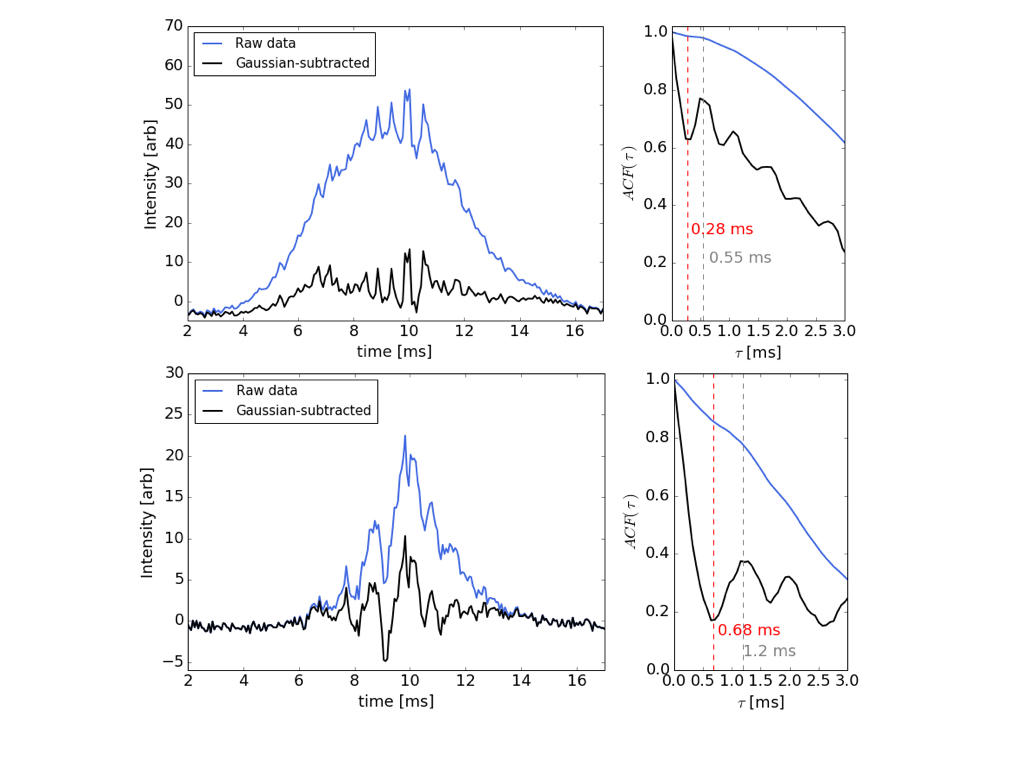
\includegraphics[trim={2in 1in 2in 0in}, width=\textwidth]{./figures/microstructure/quasi_periodicity.jpeg}
\caption{Periodicity and quasi-periodicity seen in 
     microstructure from 
     two different B0329+54 pulses, but on the same sub-pulse. 
     The top left panel shows a pulse with a periodic train of microbursts
     for both the raw profile (slate blue) and the 
     Gaussian-subtracted profile (black). The bottom 
     left panel shows broader and more moduluated 
     quasi-periodic microstructure. The right panels 
     show the corresponding ACF (slate blue) and rACF (black). 
     There are two striking features about these plots. The first 
     is that unlike other pulsars that exhibit microstructure,
     B0329+54 does not seem to have a characteristic period or width 
     to its structure. This is seen by comparing the first 
     minima and maxima of the correlation functions and 
     noticing they are at different timescales for the two 
     pulses. The second 
     is that the correlation function contains very little 
     information if a smooth component is not first subtracted, i.e., if 
     the rACF is not computed.}
\label{fig-quasistruct}
\end{center}
\end{figure}


An example of this is 
shown in the Fig.~\ref{fig-quasistruct}. The left 
panels shows bright single pulses with a
trains of microbursts for both $S(t)$ and $S'(t)$.
The right panel shows the corresponding ACFs. The 
black curve is the rACF, since it is 
the autocorrelation of a Gaussian-subtracted pulse. 

There is a known correlation between microstructure 
timescales and the pulsar period. 
\citet{2002MNRAS.334..523K} have shown the scaling to be,

\begin{equation}
t_\mu \approx 6\times10^{-4} P,
\end{equation}

\noindent where $P$ is the pulsar's period and 
$t_\mu$ is the timescale of individual microbursts, 
often estimated by the first local minimum in the ACF. 
This was consistent with the original claim by 
\citet{1979ApJ...233..981C}. 
\citet{2015ApJ...806..236M} used 24 L-band pulsars 
to revisit the relationship. Instead of using $t_\mu$, 
they used the period of quasi-periodic microstructure, 
$T_\mu$, and found it too increased 
with pulsar period as $\sim 10^{-3} P$. Here we will follow suit and 
focus primarily on the first local maximum. The reason we use
this rather than widths of individual microbursts 
is because those are often unresolved in time or scattered 
by the ISM. 

For B0329+54 we find the absence of a characteristic 
timescale, but consistency with 
the known $t_\mu-$ and $T_\mu-P$ relation. 
In Fig.~\ref{fig-quasistruct} we show 
an illustrative example of the differences in 
microstructure timescales from pulse to pulse. The 
top row's pulse has $t_\mu \sim 0.28$\,ms and 
$T_\mu \sim 0.55$\,ms, whereas the bottom row's pulse 
has $t_\mu \sim 0.68$\,ms and $T_\mu \sim 1.2$\,ms.
For B0329+54 we expect the first minima of rACFs
to be around $400$\,$\mu$s and the first maxima 
to be at $700$\,$\mu$s. In general, we find a range of 
$t_\mu \sim 100-1000$\,$\mu$s and 
$T_\mu \sim 500-2000$\,$\mu$s, which are consistent 
with the trend seen in other pulsars. 

There are two basic ways to get sub-millisecond 
variations in pulsars: angular beaming in the 
direction transverse to the observer, and actual temporal 
modulation in the magnetosphere.  
To interpret our measured timescales, we can start 
in the framework of a beaming model, in which 
the width of a micropulse is given by a 
radiating point source with some Lorentz factor, $\gamma$.
If we take $t_\mu$ as an upper limit for the 
width of a microburst, the pulse's width in radians is 
at most,

\begin{equation}
\phi = 2 \pi \, t_\mu / P\,.
\end{equation}

\noindent The Lorentz factor will be given by,

\begin{equation}
\gamma = \frac{1}{\phi\, \textrm{sin}\delta}\,,
\end{equation}

\noindent where $\delta$ is the angle between 
the pulsar's rotation axis and the line of site \citep{1998A&A...332..111L}.
Our results give a lower-limit on $\gamma$ of 
$\sim$500-1200. This is difficult to reconcile 
with several theoretical studies, which suggest 
the particles producing microstructure should have
$\gamma<100$ \citep{1992msem.coll..322A, 1998A&A...332..111L}.

In the temporal modulation picture, the effect
is not geometric but due to fluctuations in 
the intensity of waves propagating in the magnetosphere.
\citet{1983Ap&SS..97....9C} is an example of a temporal model, which 
does not require any beaming. In it, non-linear effects 
in the polar-cap plasma lead to intensity modulation 
along the radial direction.

\subsubsection{Polarized periodicity}

\citet{2015ApJ...806..236M} found that not only did 
their set of low-Galactic latitude pulsars 
have characteristic periodicities ($T_\mu$), but that 
those timescales were common across all Stokes 
parameters. Though we do not find a repeatable 
timescale in B0329+54, we do find its 
quasi-periodic microstructure to have the same 
timescales in Stokes I, V, and linear polarization.
We can see this visually 
for I and $|P_L|$ in Fig.~\ref{fig-polwaterfall}.

\citet{2015ApJ...806..236M} suggest that the similarity of 
the microstructure in 
linear and circular polarization with total intensity 
means the structures cannot be 
caused by coherent curvature radiation. 
\citet{1990A&A...234..269G} worked through the 
polarization consequences of a model 
in which the incoherent superposition of a large 
collection of sub-nanosecond pulses produced 
by the curvature mechanism resulted in pulsar radio emission.
They found the charged bunches in vacua scenario predicts
sign-changing circular polarization. Since 
\citet{2015ApJ...806..236M} do not see 
handedness switching in individual microbursts, they conclude 
that such a mechanism cannot be the source of microstructure.  
We looked for a similar effect. In sub-pulses that had both significant 
Stokes V and modulated microstructure we did not find any sign-changes, 
even when the circular polarization went from right- to left-handed
across the sub-pulse. A caveat is that we do not find any 
microstructure as heavily modulated or resolved as the pulses 
\citet{2015ApJ...806..236M} found, meaning the microbursts 
we observe could be de-polarized or the sum of multiple 
modes. Therefore we do not claim that the 
absence of a sign change in B0329+54's microstructure 
can definitively rule out charged bunches emitting 
curvature radiation as their source. Instead we simply note 
that this feature was not seen, and might have been seen 
in the coherent curvature radiation model.


\begin{figure}[!h]
\vspace{-0.1cm}
\begin{center}
\includegraphics[trim={0in 0in 0in 0in}, width=\textwidth]{./figures/microstructure/micro_pol_waterfall.png}
\caption{An example of the way the linear polarization 
     traces periodic microstructure.}
\label{fig-polwaterfall}
\end{center}
\end{figure}

\subsection{Microburst spectral variation}

In some of the brightest pulses we find frequency 
variation between individual microbursts. Given 
the timescales invovled (200-1500\,$\mu$s), such 
variation is not expected to be due to propagation 
effects like scintillation. The top right panel of 
Fig.~\ref{fig-spectralvar} shows the same pulse at 
450\,MHz (red) and 640\,MHz (black). We isolate the
three brightest individual micropulses shaded by 
light blue, light red, and grey. One can see the 
light blue pulse is quite bright at 640\,MHz, 
but less so at 450\,MHz. The light grey pulse almost 
completely disappears by 640\,MHz, even though 
it is prominent at lower frequencies. The light 
red microburst is somewhere between the other two.

In order to 
compare the frequency structure more easily, the off-pulse 
(any RFI or Galaxy in the beam) was subtracted, and the 
averaged pulse profile of B0329+54 was divided out.
This is why the spectra in the bottom panel of Fig.~\ref{fig-spectralvar}
are nearly flat. 

The difference in spectral behaviour for 
adjacent micropulses is difficult to explain 
if microstructure is caused by temporal 
variation in the magnetosphere. If each pulse is not a result 
of an individual collection of coherently emitting 
charged bunches, then why would frequency behaviour 
changed so drastically on such a short timescale?


\begin{figure}[!h]
\vspace{-0.5cm}
\begin{center}
\includegraphics[trim={1.8in 0in 1.in 0in}, width=\textwidth]{./figures/microstructure/spectra.jpeg}
\caption{An example of broad-band microstructure in a 
particularly bright pulse. This pulse's three most prominent 
microbursts have very different frequency behaviour. \textit{top left:}
Frequency time colour map showing this pulse over the 
full band, for roughly 15 ms. The broad-band nature of 
the microstructure is also apparent as 
vertical pipe-like structures. \textit{top right:} Pulse 
profile for two different frequencies: centered on 640\,MHz and 450\,MHz, 
averaged over $\sim$40\,MHz. The three vertical shaded regions, 
blue, red, and grey, correspond to the three brightest 
micropulses, ``micropulse 1", ``micropulse 2", ``micropulse 3", 
respectively. One can also see their differences in their 
spectral behaviour. The first spike is brighter at 450\,MHz
than at 640\,MHz, but the opposite is true of the
second and third spikes. \textit{bottom panel:} The relative 
spectra of three micropulses, with colours corresponding 
to the shaded region in the top right panel.}
\label{fig-spectralvar}
\end{center}
\end{figure}

% \subsection{Microstructure and DM}
% Variation in DM leads to significant uncertainty in pulse
% time-of-arrival (TOA). Folded spectra from slow 
% pulsars provide a profile that is 
% too broad to precisely measure DM. Microstructure, on
% the other hand, can be as narrow as pulses from 
% millisecond pulsars (MSPs).


% \begin{figure}[!h]
% \begin{center}
% 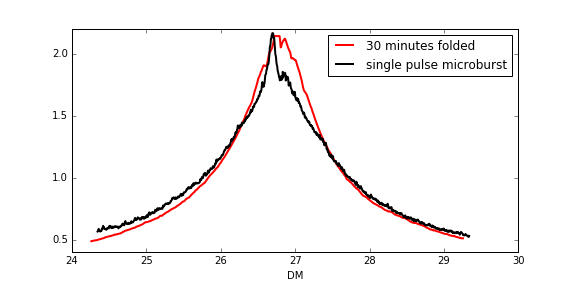
\includegraphics[trim={0.in 0in 0.in 0in}, width=\textwidth]{./figures/microstructure/DM_from_folded_pulse.png}
% \vspace{0.0cm}
% \caption{}
% \label{fig-micro}
% \end{center}
% \end{figure}



\section{Conclusion}
\label{sec:conclusion}
  
We have presented analysis of the largest collection 
of single-pulse microstructure data of 
B0329+54. Broadband microstructure was found to be a 
generic property of this pulsar, although it is
rarely highly modulated. The sub-pulses we analyzed often 
exhibited quasi-periodic trains of micropulses. We 
quantified such periodicity with a reduced autocorrelation 
function, which pulls out time-like correlations by 
first removing the stronger, smooth component of the 
sub-pulse. The quasi-periodic microstructure of B0329+54
were found to have no characteristic timescale, which is
different from other pulsars that have been studied. 
However, we did show that the range of periods are 
consistent with the known $T_\mu \approx 10^{-3}\,P$ relation. 
The micropulse widths are also roughly consistent with 
the known $t_\mu-P$ scaling. These scalings held for 
the polarized microstructure as well. Linear polarization 
and Stokes V were both found to mimic total intensity in 
their quasi-periodicities. As \citet{2015ApJ...806..236M} 
have shown, one would not necessarily expect this 
if the microstructure came from 
coherent curvature radiation of charged bunches.

The microburst widths allow us to estimate the Lorentz 
factor of the radiating particles, assuming the widths 
are due to relativistic beaming. We find $\gamma\sim500$-$1200$, 
which are inconsistent with the expected velocities. 
This inconsistency was also found by \citet{1998A&A...332..111L}, 
who use it to reject the beaming model. The other standard 
explanation for the origin of pulsar microstructure is not 
geometric but temporal. The idea is that time-like 
fluctuations in the magnetospheric plasma generate the 
periodic and quasi-periodic trains of sub-millisecond pulses
that are observed in a number of sources. 

In the framework of this model, we found the spectral 
behaviour of B0329+54's microstructure to be difficult
to interpret. In several strong pulses we found 
micropulses within a single sub-pulse to have very different 
broad-band frequency characteristics. If the pulses 
do not come from physically separate collections of 
charges, then we would not expect vastly different 
spectral properties. 


%\include{./sections/conclusions}

% ==============================================================================
% BIBLIOGRAPHY
% ==============================================================================

\addcontentsline{toc}{chapter}{Bibliography} % Adds a line for the Bibliography in the Table of Contents.

\bibliographystyle{apj}
\bibliography{references}

\end{document}
